\documentclass [a4paper] {article}

\usepackage[spanish]{babel} 
\usepackage[utf8]{inputenc} 
\usepackage{multirow} 
\usepackage{float} 

\title{R-PL6}
\author{Gabriel López Cuenca, Sergio Sanz Sacristán, Álvaro Zamorano Ortega}

\usepackage{Sweave}
\begin{document}
\Sconcordance{concordance:G16-p6.tex:G16-p6.Rnw:%
1 10 1 1 0 16 1 1 2 1 0 3 1 3 0 1 2 6 1 1 2 4 0 1 2 2 1 1 2 1 0 1 1 3 0 %
1 2 3 1 1 2 1 0 1 1 1 2 1 1 3 0 1 2 6 1 1 2 1 0 2 1 3 0 1 2 4 1 1 2 1 0 %
3 1 3 0 1 2 6 1 1 2 1 0 3 1 3 0 1 2 5 1 1 2 1 0 2 1 3 0 1 2 5 1 1 2 1 0 %
2 1 3 0 1 2 5 1 1 2 1 0 2 1 3 0 1 2 3 1}


\maketitle

\graphicspath{ {./tmp/} }

\section{Visualización.}

\subsection{Salarios medios mensuales en Europa.}
\bigskip
Hemos hecho un tratamiento de datos correspondiente a los salarios medios mensuales de los países europeos.
Lo que buscamos es representar el conjunto de datos de estos salarios medios, para localizar, de forma clara
y sencilla la posición actual de España con respecto al resto de los países de su alrededor.

\bigskip
Para llevar a cabo esto lo primero que realizamos es importar los datos correspondientes:
\begin{Schunk}
\begin{Sinput}
> install.packages("readr")
> library("readr")
> datos <- read_csv("paises.csv")
> datos <- data.frame(datos)
\end{Sinput}
\end{Schunk}

\bigskip
Para que el diagrama quede lo más claro posible vamos a realizar un \textbf{diagrama de Pareto}. Un diagrama
de Pareto es un tipo especial de gráfica de barras donde los valores graficados están organizados de mayor a 
menor. Se utiliza para para identificar los defectos que se producen con mayor frecuencia, las causas más 
comunes de los defectos o las causas más frecuentes de quejas de los clientes. Por lo tanto, ordenamos los
datos de mayor a menor:
\begin{Schunk}
\begin{Sinput}
> datos$Pais <- factor(datos$Pais,levels=datos$Pais[order(datos$Salario)])
\end{Sinput}
\end{Schunk}

\bigskip
Para representar el diagrama utilizaremos el paquete \textbf{ggplot2}. Lo instalamos y lo inicializamos.
\begin{Schunk}
\begin{Sinput}
> install.packages("ggplot2")
> library("ggplot2")
\end{Sinput}
\end{Schunk}

\bigskip
Inicializamos el diagrama e introducimos los datos. Inicialmente nos saldrán los datos en barras verticales, y
de diferentes colores al llamar a la función \texttt{geom\_bar}.
\begin{Schunk}
\begin{Sinput}
> sp <- ggplot()
> sp <- sp + geom_bar(data=datos,aes(x=datos$Pais, y=datos$Salario,fill=datos$Pais), stat='identity', position='dodge',show.legend=FALSE)
> source("./Funciones/diagrama.R")
> diagrama("diagrama1.png",sp)
\end{Sinput}
\end{Schunk}

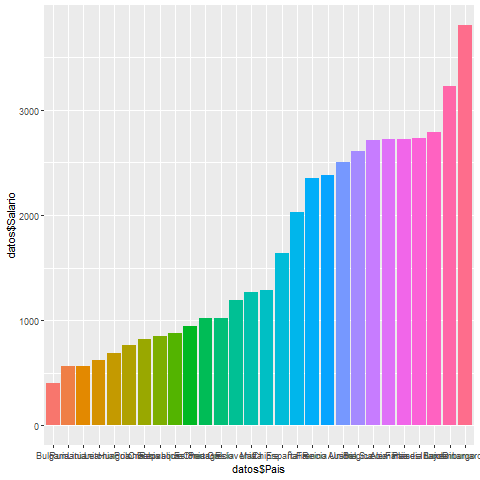
\includegraphics[width=\textwidth]{diagrama1}

\bigskip
Ya que los datos son identificados por nombre, es recomendable que estos se coloquen de la forma más visible
posible. Por lo tanto, lo que hacemos es rotar el diagrama para que queden los nombres en el eje y, y así
sean mucho mas visibles. Pasamos las barras de vertical a horizontal.
\begin{Schunk}
\begin{Sinput}
> sp <- sp + coord_flip()
> source("./Funciones/diagrama.R")
> diagrama("diagrama2.png",sp)
\end{Sinput}
\end{Schunk}

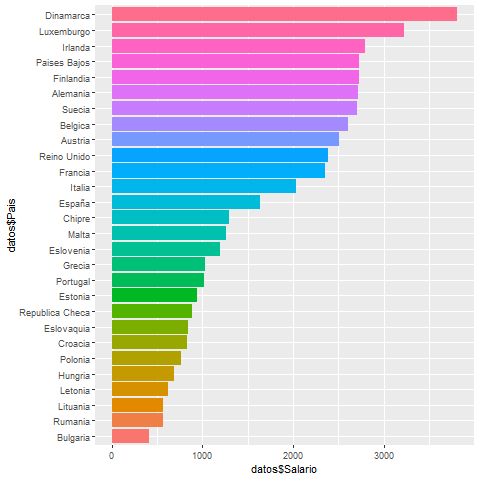
\includegraphics[width=\textwidth]{diagrama2}


\end{document}
